\documentclass{standalone}
\usepackage{pgfplots}
\pgfplotsset{compat=1.11}
\begin{document}
% Place the TikZ picture in a figure environment.
%\begin{figure}[htb]
% h: here, t: top, b: bottom, p: page of float
%% https://tex.stackexchange.com/questions/39017/how-to-influence-the-position-of-float-environments-like-figure-and-table-in-lat
%% ! indicates that some restrictions should be ignored (discussed later)
%% h indicates that the float is allowed to be placed inline
%% t indicates that the float is allowed to go into a top area
%% b indicates that the float is allowed to go into a bottom area
%% p indicates the the float is allowed to go on a float page or column area

    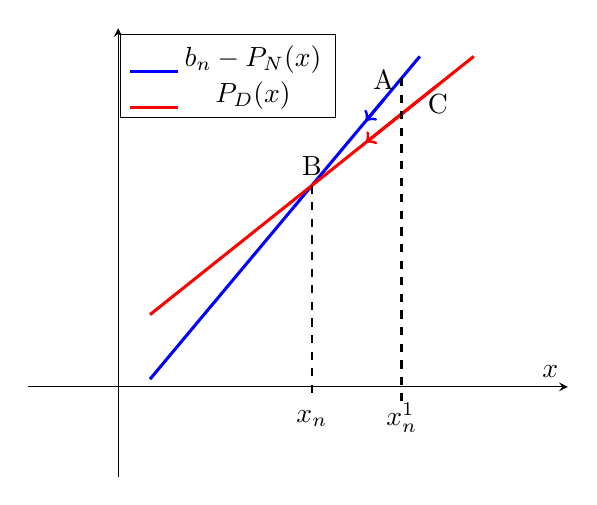
\begin{tikzpicture}
        \begin{axis} [
            xmin=-0.5, xmax=2.5, ymin=-0.5, ymax=2, 
            xlabel={$x$},
            % xtick={-2,-1.5,...,2}, ytick={-2,-1.5,...,2},
            xticklabel style={font=\tiny, xshift=0.5ex},
            yticklabel style={font=\tiny, yshift=0.5ex},
            axis line style={->},
            axis x line=middle,
            axis y line=middle,
           % legend pos=north west,
           ticks=none,
           legend style={at={(0.17,0.8)},anchor=south west}
        ]
        % \addplot+[mark=none, line width=1.1, color=blue, domain=-2:-0.5] {x+0.5};
        % \addplot+[mark=none, line width=1.1, color=blue, domain=-0.5:0.5] {0};
        \addplot+[mark=none, line width=1.1, color=blue, domain=0.1:1.6][xshift=5pt,yshift=-5pt] {1.2*x};
        
        \addplot+[mark=none, line width=1.1, color=red, domain=0.1:1.9][xshift=5pt,yshift=-5pt] {0.8*x + 0.4};
        % \addlegendentry{$k=1$}
        
        % \node[below] (A) at (0.3, 0.36) {A};
         \node[below][xshift=5pt,yshift=-5pt] (C) at (1.7, 1.76) {C};
        
        \node[above][xshift=5pt,yshift=-5pt] (B) at (1, 1.2) {B};
        % \node[above] (C) at (0.3, 0.64) {C};
        \node[above][xshift=5pt,yshift=-5pt] (A) at (1.4, 1.68) {A};
        \node[below][xshift=5pt,yshift=-5pt] (xn) at (1.5, 0.04) {$x^{1}_n$};
    \node[below][xshift=5pt,yshift=-5pt] (xn) at (1, 0) {$x_n$};

        % \node[below] (PD) at (1.7, 1.76) {$P_D$};
        % \node[above] (PN) at (1.4, 1.68) {$P_N$};

        % \addplot[->,line width=1.1,color=blue] coordinates {(0.3, 0.36)  (0.7, 0.84)};
        % \addplot[->,line width=1.1,color=red] coordinates {(0.3, 0.64)  (0.7, 0.96)};

        \addplot[->,line width=1.1,color=red][xshift=5pt,yshift=-5pt] coordinates {(1.7, 1.76)  (1.3, 1.44)};
        \addplot[->,line width=1.1,color=blue][xshift=5pt,yshift=-5pt] coordinates {(1.4,1.68)  (1.3, 1.56)};

        \addplot[dashed,line width=1, color=black][xshift=5pt,yshift=-5pt] coordinates {(1, 1.2)  (1,0)};
        \addplot[dashed,line width=1, color=black][xshift=5pt,yshift=-5pt] coordinates {(1.5, 1.8)  (1.5,0)};

        \addlegendentry{$b_n - P_N(x)$}
        \addlegendentry{$P_D(x)$}

        \end{axis}
    \end{tikzpicture}

\end{document}